\documentclass{tufte-handout}
% \documentclass{article}

%\date{28 March 2010} % without \date command, current date is supplied

% \geometry{showframe} % display margins for debugging page layout

\usepackage{graphicx} % allow embedded images
  \setkeys{Gin}{width=\linewidth,totalheight=\textheight,keepaspectratio}
  \graphicspath{{graphics/}} % set of paths to search for images
\usepackage{amsmath}  % extended mathematics
\usepackage{booktabs} % book-quality tables
\usepackage{units}    % non-stacked fractions and better unit spacing
\usepackage{multicol} % multiple column layout facilities
\usepackage{lipsum}   % filler text
\usepackage{fancyvrb} % extended verbatim environments
  \fvset{fontsize=\normalsize}% default font size for fancy-verbatim environments
\usepackage{listings}
\usepackage{verbatim}

% Standardize command font styles and environments
\newcommand{\doccmd}[1]{\texttt{\textbackslash#1}}% command name - - adds backslash automatically
\newcommand{\docopt}[1]{\ensuremath{\langle}\textrm{\textit{#1}}\ensuremath{\rangle}}% optional command argument
\newcommand{\docarg}[1]{\textrm{\textit{#1}}}% (required) command argument
\newcommand{\docenv}[1]{\textsf{#1}}% environment name
\newcommand{\docpkg}[1]{\texttt{#1}}% package name
\newcommand{\doccls}[1]{\texttt{#1}}% document class name
\newcommand{\docclsopt}[1]{\texttt{#1}}% document class option name
\newenvironment{docspec}{\begin{quote}\noindent}{\end{quote}}% command specification environment

\begin{document}

\title{MAE-253: Homework 3a}
\author[John Karasinski]{John Karasinski}
\maketitle% this prints the handout title, author, and date

\section{A proposed outline for our project}

\subsection{Write a 2-3 sentences with the goal of the project.}
We are looking to perform community detection in online information sharing communities (such as Reddit, StackExchange, and HackerNews), and to compare network properties across different communities. One phenomena in online communities is Eternal September, when the popularity of a community reaches a critical threshold beyond which no central core of the members are in control. We're looking to build networks from the commenting and tagging dynamics contained within these communities, and detect differences between them and how they change over time.

\subsection{Outline your plan of attack, and give preliminary results.}

\begin{enumerate}
\item Download/scrape datasets.
\item ``Clean'' datasets. Remove non-human users (bots), posts with inadequate/missing information.
\item Create a network from the comment structure. A weighted, directed network can be created (user $B$ commented on user $A$'s content $N$ times).
\item Break users into `cohorts` by when users first interacted with the community. For example, a user that first interacts with the community win 2006 would be placed in the 2006 cohort, and so on for users that first post in different years. We plan to follow a procedure similar to Barbosa, Samuel, et al.~\footnote{Barbosa, Samuel, et al. ``Averaging Gone Wrong: Using Time-Aware Analyses to Better Understand Behavior.'' Proceedings of the 25th International Conference on World Wide Web. International World Wide Web Conferences Steering Committee, 2016.}
\item How do users in different cohorts interact with the community? Does the behavior of users within a cohort change over time? How do different cohorts interact with the community? Can we detect the effects Eternal September based off of differences in the cohorts?
\item Run community detection on resulting network.
\item Temporal changes of communities by cohort.
\item What network properties change by cohort? Can we draw conclusions based on these changes? Do these results correlate with the results we see in 5.?
\end{enumerate}

So far
\begin{enumerate}
\item I have scraped all the data from HackerNews's API from their creation in October 2006 up until May 1st, 2016.
\item This data has been processed to remove users with `bot-like' names. The data has been stored in csv files in the format: \\\texttt{post\_id, post\_author, parent\_id, post\_timestamp}
\item I have identified 9,125,366 comments (edges) and 253,039 unique authors (nodes) in the data. I have also iterated through to identify the authors of each comment.
\item I have identified `active users' as those users in a cohort which commented during a period of time. I then looked at monthly active users in each cohort over time to investigate the evolution of the community over time. I've identified the number of active users in each cohort over time, the number of comments from active users in each cohort over time, and the average number of comments from active users over time. See Figure~\ref{fig1}.
\begin{figure}
  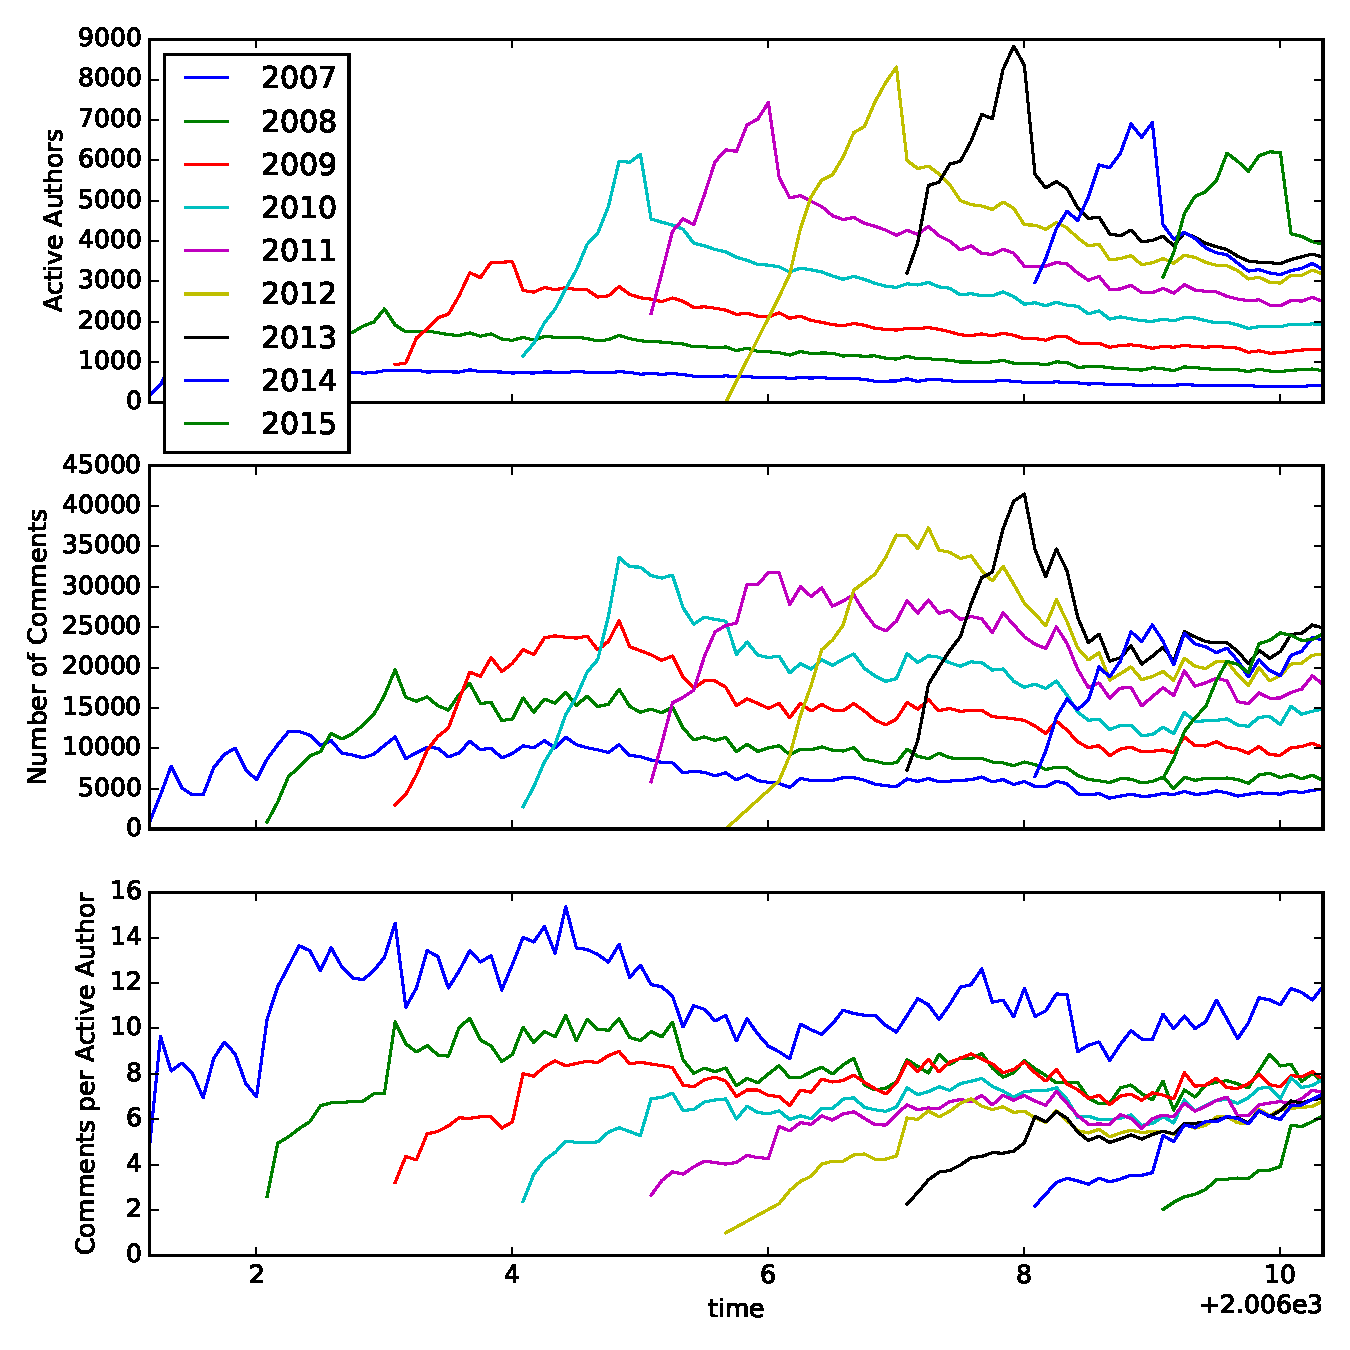
\includegraphics{stats.pdf}
%  \checkparity This is an \pageparity\ page.%
  \caption{Number of active users, comments, and average number of comments per active user in each cohort by month from 2006 to 2016. These plots suggest that there are an increasing number of active users in cohort. New cohorts tend to take some time to catch to the same level of community interaction as older users. New cohorts also seem to be unable to catch up to the original 2007 cohort, which consistently interacts with the community more than newer cohorts.
  % \emph{Notice that this figure only takes up the main textblock width.}
  }
  \label{fig1}
  %\zsavepos{pos:textfig}
  \setfloatalignment{b}
\end{figure}
\end{enumerate}

\subsection{Itemize the stumbling blocks you foresee that will keep you from achieving the desired outcome.}

\begin{enumerate}
\item It is unclear which community detection algorithms will be the most effective at detecting subcommunities within HackerNews.
\item HackerNews does not have any inherent, explicit community structure, and before doing any network analysis it is unclear if there will be any obvious structure. According to the Hacker News Guidelines\footnote{
What to Submit\\
On-Topic: Anything that good hackers would find interesting. That includes more than hacking and startups. If you had to reduce it to a sentence, the answer might be: anything that gratifies one's intellectual curiosity.\\
Off-Topic: Most stories about politics, or crime, or sports, unless they're evidence of some interesting new phenomenon. Videos of pratfalls or disasters, or cute animal pictures. If they'd cover it on TV news, it's probably off-topic.\\ \noindent \url{https://news.ycombinator.com/newsguidelines.html}}, the on-topic site topic is ``anything that gratifies one's intellectual curiosity''. This topic tends to move with current political topics and startup scene, and so temporal topics might be more evident than specific subgroups of users.
\item HackerNews is a relatively small community compared to other communities such as Reddit, which has many more users. The effects of Eternal September may not be prevalent or even present. If this is the case we can still investigate the differences between different networks (ie, HackerNews and Reddit).
\end{enumerate}

\end{document}








